\subsection{Experiment setup}
\label{sec:experiment_setup}
% \begin{figure}[t]
% 		\centering
% 		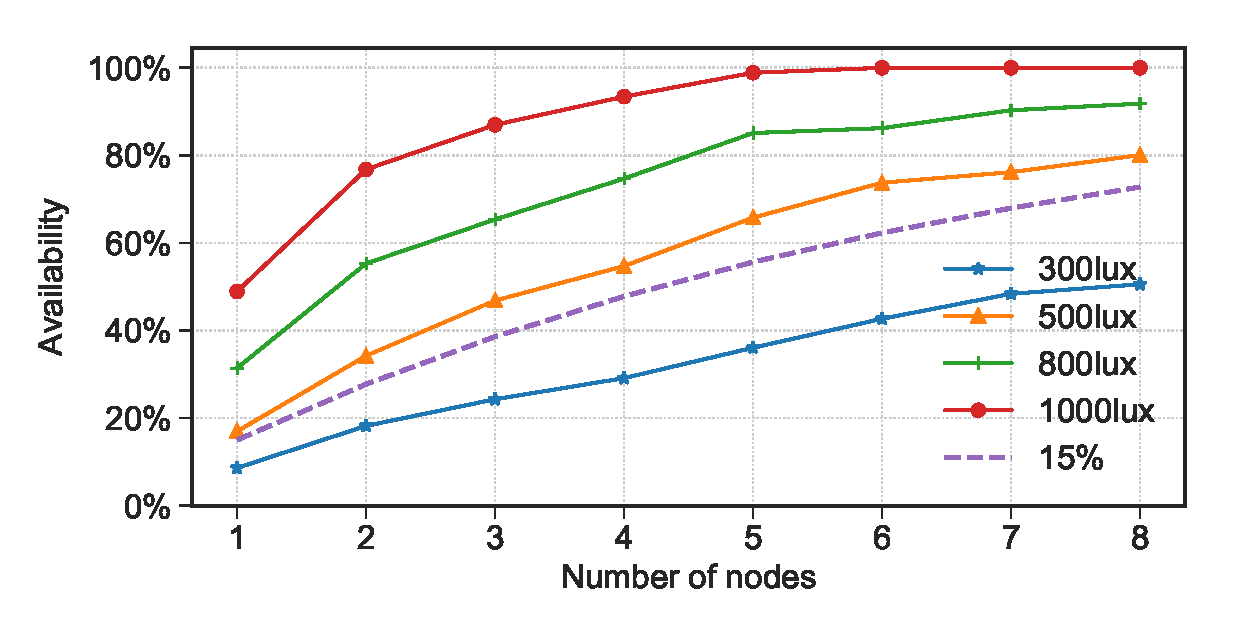
\includegraphics[width=\columnwidth]{figures/sysAvailability_artificial-light}
% 		\caption{\todo{can be removed, or merged with \sys availability figure with solar power or updated it and presented it} Implicit \fullsys' nodes distribution using artificial light power harvesting randomization}
% 		\label{fig:solarPwrCoIS}
% \end{figure} 
\begin{figure}[t]
		\centering
		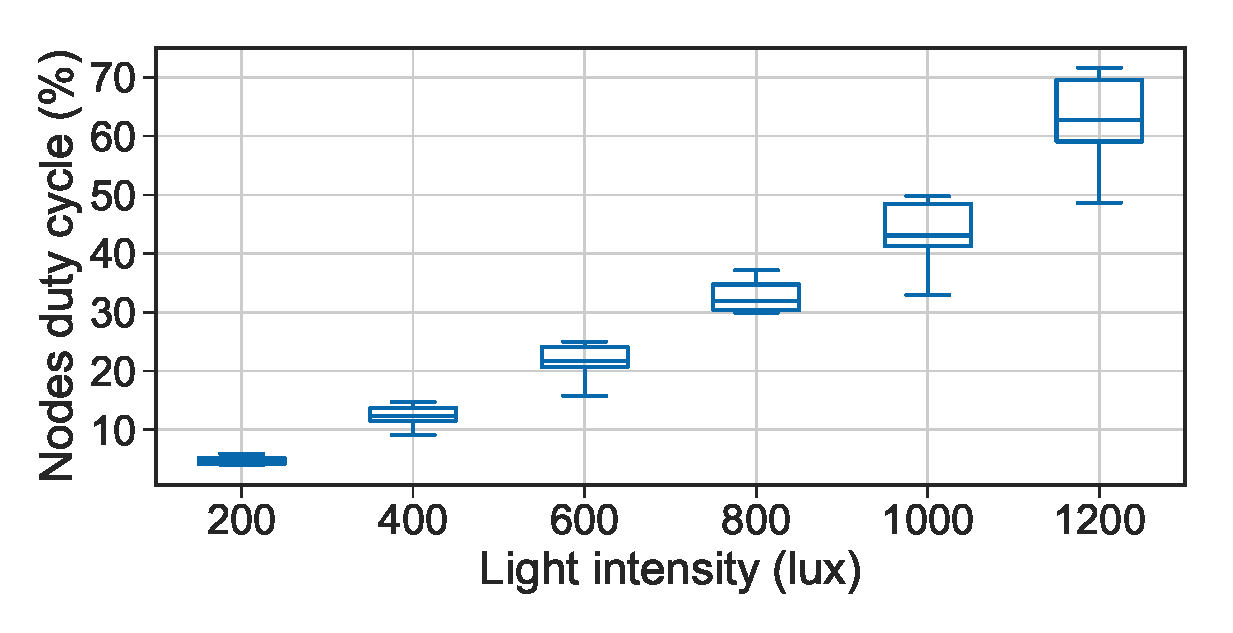
\includegraphics[width=\columnwidth]{figures/cis_dutyCycle.eps}
		\caption{\fullcim availability while being in a sleep mode for different light intensity \todo{re-discuss with Patrick the meaning of this figure}}
		\label{fig:cis_dutyCycle}
\end{figure} 
\begin{figure}[t]
		\centering
		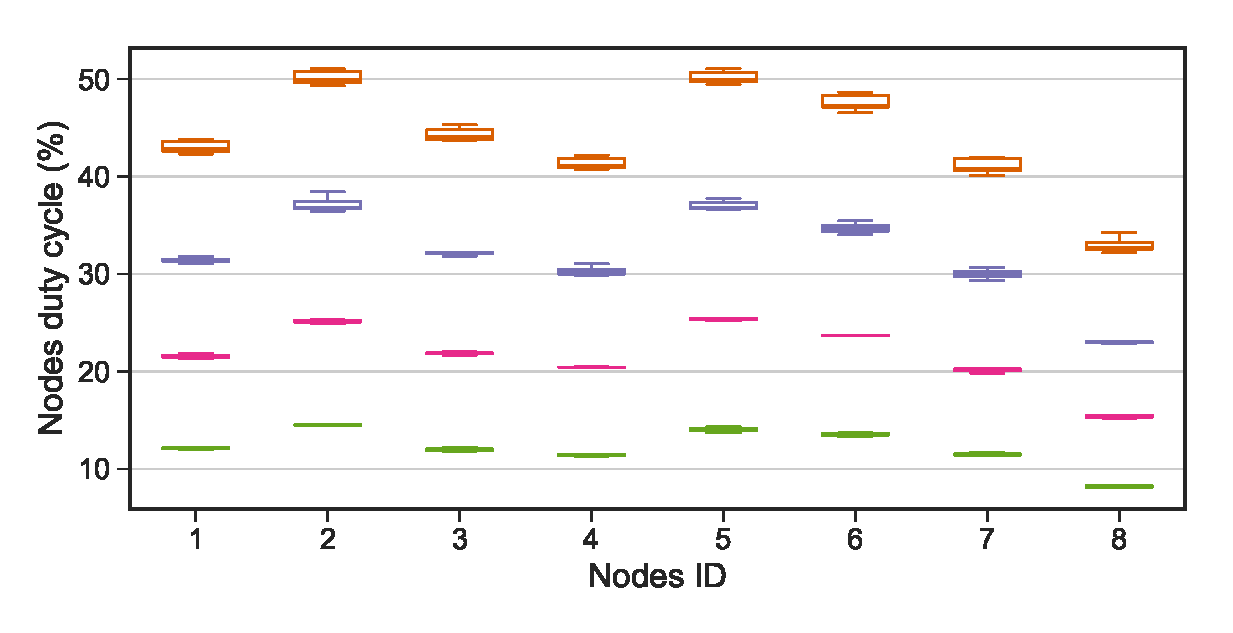
\includegraphics[width=\columnwidth]{figures/nodes_duty_cycles.eps}
		\caption{\fullcim nodes' duty cycles for a artificial light intensity ranges from $\approx 400$ to $\approx \SI{1000}{lux}$}
		\label{fig:solarPwrCoIS}
\end{figure} 
After validating our observation on natural light and office artificial light, we designed a testbed with controllable light intensity for clarity and results reproducible. We blocked uncontrollable light sources with a box of $60 \times 40$\,cm. On one side we fix a light strip of 2.5\,m with 150 LED~\cite{}. On the other side is the \fullcim of 8 intermittent nodes. The light strip can produce 16 difference light intensity. Figure~\cite{fig:cis_dutyCycle} shows the \cim power cycles while being in low-power-mode for a light intensity ranges from a minimum ($\approx 100$\,lux) to a maximum ($\approx 2000$\,lux). 

\subsection{Events detection rate}
In these experiments we study the reaction behavior to the \sys for bursty and regular events.
\paragraph{Regular events arrival}
\begin{figure}[t]
		\centering
		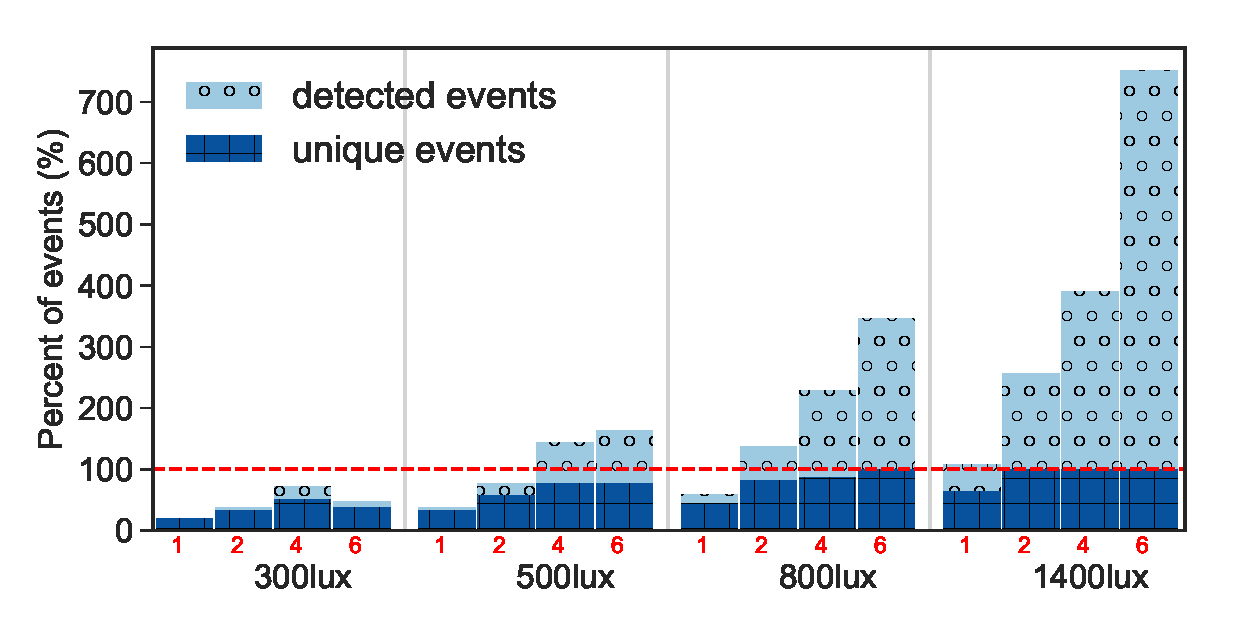
\includegraphics[width=\columnwidth]{figures/regular_events_capture_rate.eps}
		\caption{The number of detected events by \fullcim with eight intermittent nodes. The total number of the external events is 240. In general, we see that when the light intensity increases, the number of captured events rises too. But... \todo{add timing, and possibly inject bars with randomization }}
		\label{fig:events_detection_rate}
\end{figure}

Figure~\ref{fig:events_detection_rate} shows the rate of unique events detection and the total detection rate, for four different light intensity. We clearly see a positive correlation between light intensity and the number of duplicated events. We also observe that the number of duplicated detected events increases when the arrival time between the events is longer. The reason for this phenomena is that when the inter-events time increases, the intermittent nodes sleeps longer in low-power-mode. This reduces the inherent randomization of the system and leads it to the \textit{hibernating-power-state} problem and eventually to the \textit{overpowering} problem (Section\ref{sec:power_state}).  
 

\paragraph{Bursty events arrival}
\begin{figure}[t]
		\centering
		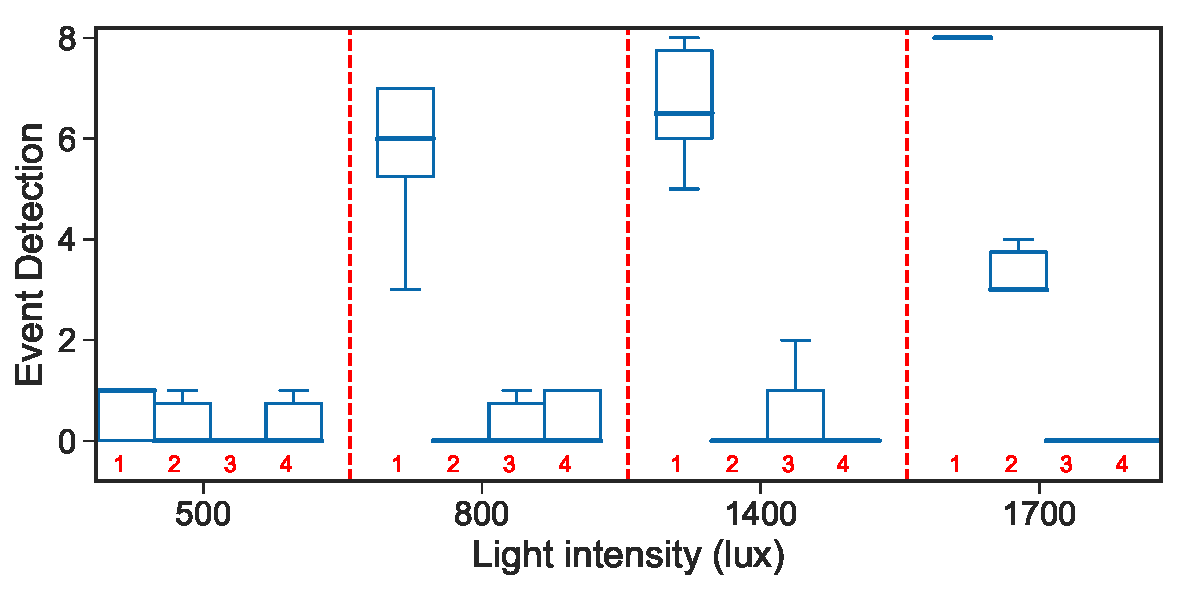
\includegraphics[width=\columnwidth]{figures/events_burst_problem.pdf}
		\caption{when the system sleeps, randomization is reduced. Thus, the majority of the nodes react to the first event and miss the rest of the burst. Red numbers indicate events index in a burst}
		\label{fig:events_burst_problem}
\end{figure} 
Figure~\ref{fig:events_burst_problem} shows the capturing behavior of \sys of a bursty-type events. A bust of four events with one second between the individual events were fired every 20 seconds. Each burst was repeated 10 times. The nodes sleep in low-power-mode when they finish processing waiting or the next event. In general, we observe that the intermittent nodes react to the first event and power down shortly after missing the rest of the burst. The results validate our theory about the side effect of the \textit{hibernating power state} (Section~\ref{sec:power_state}). Next we will show how randomized response can mitigate this problem. \todo{what is the total captured event numbers? to be compared to the total captured event numbers with randomization}


\subsection{Events detection rate with randomization}
\begin{figure}[t]
		\centering
% 		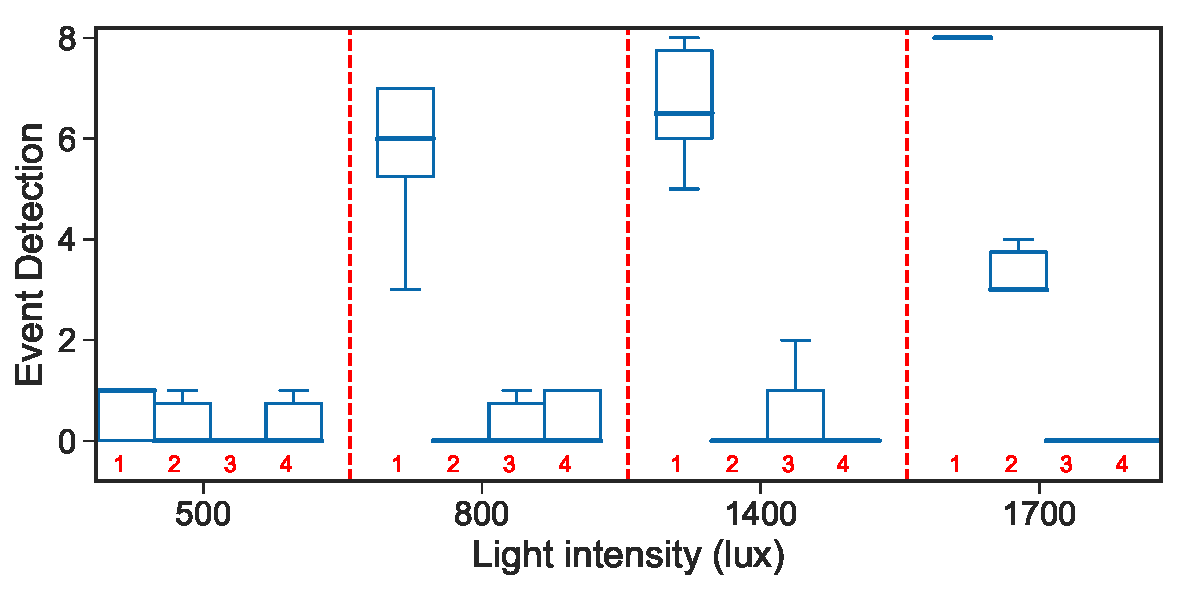
\includegraphics[width=\columnwidth]{figures/events_burst_problem.pdf}
		\caption{\todo{Figure to show how randomization helps in increasing the uniquely detected events rates}}
		\label{fig:solarPwrCoIS}
\end{figure} 


\begin{figure}[t]
		\centering
% 		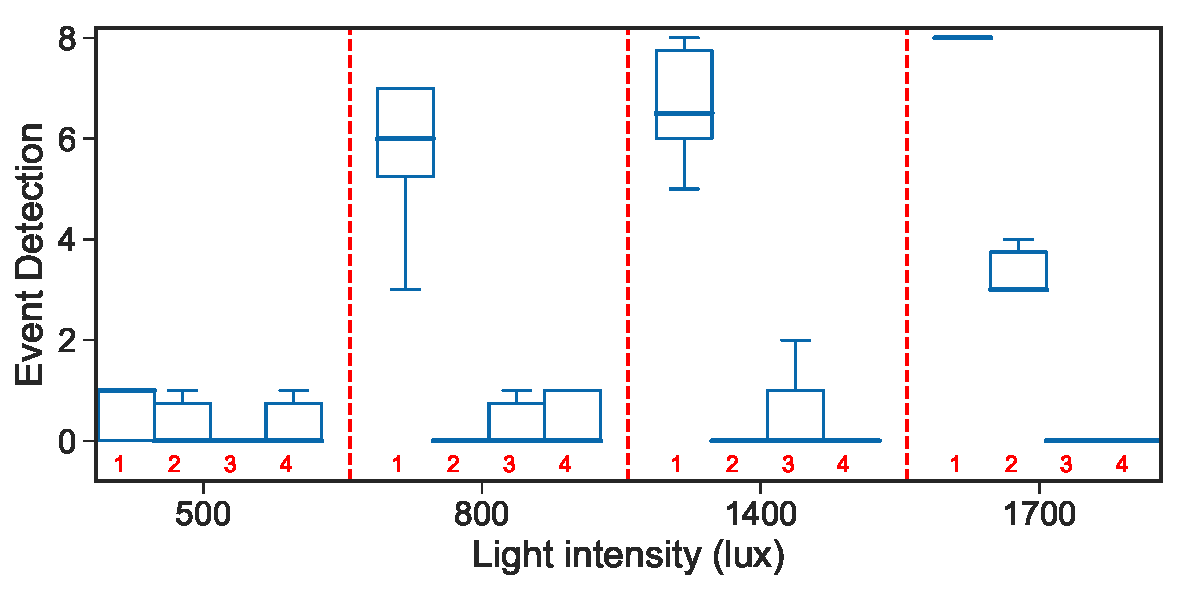
\includegraphics[width=\columnwidth]{figures/events_burst_problem.pdf}
		\caption{\todo{Figure to show how randomization help in mitigating the bust problem}}
		\label{fig:solarPwrCoIS}
\end{figure} 

\subsection{\fullcim words detection accuracy}
\begin{table}[H]
\centering
\caption{Testing set}
\label{tab:words}
\begin{tabular}{lllll}
\hline
on    & off  & stop & clear & load   \\
go & pause & resume & edit  & quit  \\  
\hline  
\end{tabular}
\end{table}


\subsection{ Intermittent microphone availability}
%
\todo{BELOW ID OLD WORK}
\begin{figure}
\centering
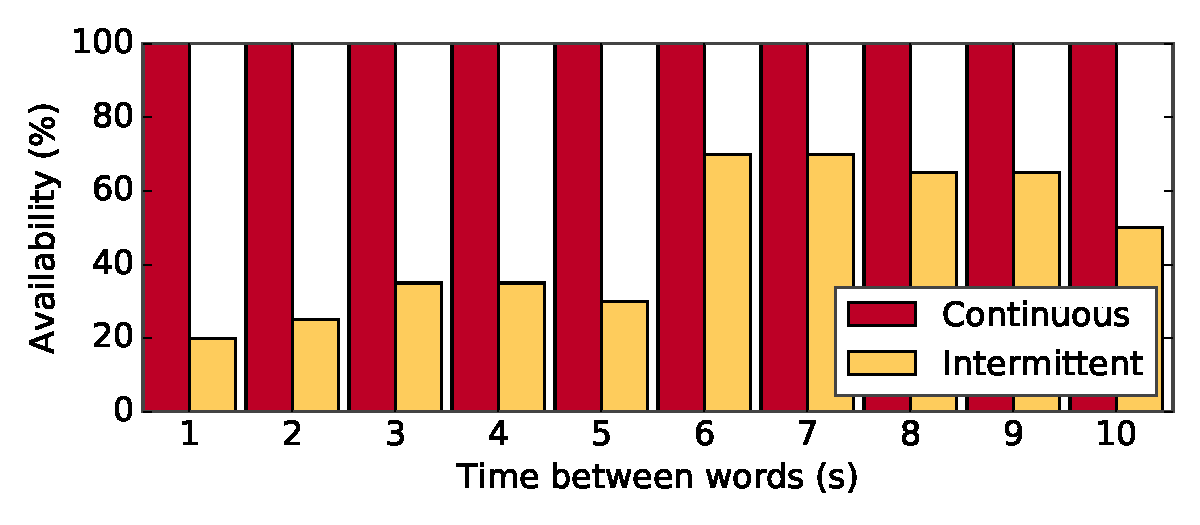
\includegraphics[width=\linewidth]{figures/word_freq}
\caption{\todo{These are old results} The effect of the time between consecutive words on the availability: the percentage of words that is processed by the command recognizer. \todo{Add correct recognition as stacked bar?}}
\label{fig:word_freq}
\end{figure}
%
\begin{table}
	\centering
	\caption{The mean and standard deviation of the parameters that were used to simulate intermittent execution. Here $t_{on}$ is the time the device is on while recording or processing, $t_{off}$ is the time the device is charging and $t_{sleep}$ is the time the device is sleeping while waiting on sound input.}
	\label{tab:simparams}
$
\begin{array}{lll}\hline
\text{Parameter} & \mu \text{ (ms)} & \sigma \text{ (ms)} \\\hline
%t_{rec} & 295 & 0 \\
t_{on} &  590 & 17.7 \\
t_{off} & 5310 & 154 \\
t_{sleep} &  22420 & 652 \\\hline
\end{array}
$
\end{table}
%
This experiment shows the effect of intermittent power supply on a microphone availability \todo{and recognition accuracy} for different command (or word) repetition speed. Each word (from Table~\ref{tab:words}) was played back 20 times with intra-words-playing time ranges from 1 to 10 seconds. 

For the experiment we chose to simulate the intermittent power supply, based on a real measurement, to ensure environment consistency across different words.
In particular, we measured the $t_{on}$; used an on/off ratio of $10\%$ to simulate harsh harvesting conditions~\cite{mementos, bhatti2017harvos,lucia}; and calculated the $t_{sleep}$ based on the micro controller specification~\cite{datasheet} (Table~\ref{tab:simparams}).     

The obvious observation from Figure~\ref{fig:word_freq} is that intermittency has a great impact on the command recognizer availability. However, a less obvious, but important, observation is that the correlation between the on/off cycle and the command repetition speed has also great impact as the bars labeled with 5 and 6 from Figure~\ref{fig:word_freq} indicate. 





